Classic mixture models make the assumption that the data are drawn
from a finite collection of distributions. A data point is generated
by first selecting one of the distributions, and then drawing a
sample. In this model, the data $X^n$ are observed and the cluster
indicators $Z^n$, cluster mixture weights $\pi_{1:K}$ and the
parameters of the distributions $\theta_{1:K}$ are hidden. Such models
are useful for clustering, since we can infer the hidden cluster
indicators $Z^n$ to recover a partition of the data that is likely
according to the generative story sketched above.

While mixture models are useful and can act as fundamental components
of more sophisticated hierarchical models, it is often difficult in
practice to choose the correct number of clusters $K$ that should be
used. This is known as model selection, and is often done by learning
models for a variety of $K$ and assessing the fit of each model using
a metric such as held-out log likelihood or Akaike information
criterion.

An alternative to model selection is to use Bayesian nonparametric
models such as the Dirichlet process mixture model \cite{antoniak1974}
which assumes \textit{a priori} that there are an infinite number of
clusters (i.e. $K \to \infty$). While theoretically infinite, the
Dirichlet process generates mixture weights $\pi_{1:\infty}$ over the
clusters where finitely many of the clusters have non-zero
probabilities. While there is no known density function for this
distribution, there are several algorithms available that can sample
from the Dirichlet process, which makes this powerful model usable in
practice.

The generative story for a DP mixture model is the following. A
single, finite dimensional, categorical distribution $G$ is drawn from
the Dirichlet process $DP(\alpha, H)$. The DP is parameterized by the
base distribution $H$ and the concentration parameter $\alpha$. The
concentration parameter can be compared to the concentration parameter
of a Dirichlet distribution. In the symmetric Dirichlet, $\alpha$
controls how much draws from the distribution will vary from the
$K$-dimensional uniform categorical distribution. For example, $\alpha
= 0.1$ will result in sparse distributions because we are saying that
draws from the Dirichlet should not be concentrated around the uniform
distribution. On the other hand, when $\alpha = 10$, draws will
frequently be close to uniform. Analogously, the concentration
parameter of the DP will influence how similar $G$ is to $H$. If
$\alpha$ is low, then $G$ will put the majority of its probability
mass on several samples from $H$. If $\alpha$ is high, then $G$ will
have a wider support, with probability distributed over the support in
a way that is similar to $H$. Conditioned on the draw $G$, for each
point $X_i$, we draw a set of parameters $\theta_i$ from $G$. Note
that $G$ is a discrete distribution, and so we will frequently
resample the same parameters. Given a set of parameters $\theta_i$,
$X_i$ is sampled from the distribution $f(\theta_i)$. In math, this
can be expressed as

\begin{align}
  G &\sim DP(\alpha, H) \\ \theta_i|G &\sim G \\ X_i|\theta_i &\sim f(\theta_i)
\end{align}

In the DP mixture model, we are interested in inferring the cluster
indicators $Z^n$ (equivalently the partition of the data $\Pi$) and
the parameters $\theta_{1:|\Pi|}$ associated with each cluster. We are
rarely interested in the random measure $G$, which is often
marginalized out. When marginalized out, we can use the Chinese
Restaurant Process to do inference over the cluster indicators $Z^n$
and the parameters $\theta_{1:|\Pi|}$.

\subsection{The Goldwater model as a DPMM}

A key insight that allowed us to parallelize the Goldwater model was
that the model can be reformulated as a DP mixture model. Recall that
the key components of a DPMM are the base distribution $H$ over
parameters, and a family of distributions $\mathcal{F}$ indexed by the
parameters in the support of $H$.

The Goldwater model uses a DP to dampen the counts observed in a
corpus. Type frequencies in a corpus of natural text are often highly
skewed---i.e. some types occur very frequently while the majority
occur infrequently. This phenomona also occurs among the different
inflections of the same lexeme. For example, the first-person, present
tense inflection \textit{walk} may occur much more frequently than
\textit{walked} in a particular corpus. In languages with many
different inflections for a particular \textit{lexeme} this can be
especially problematic. Since it is important to learn all
grammatically valid inflections of a word, the DP normalizes token
frequencies so that inflections that are used more often are do not
bias model estimation.

With this in mind, the DP is used as an \textit{adaptor}
\cite{goldwater2011}, and not as a distribution over measures over
parameters. If we notice, however, that the base distribution $H(w)$
in the goldwater model is defined to be

\begin{align*}
  H(w) &= \sum_{(p,s) \in segs(w)} p(p | \theta_p) p(s | \theta_s)
\end{align*}

which we can view as the marginal distribution of $w$ in a mixture
model where $(p,s)$ are parameters indexing a point distribution over
words where the probability of $w = p + s$ is $1$ and all other words
have probability $0$. With this in mind, we can then redefine the
generative story of the Goldwater model as follows

\begin{align*}
  \theta_p & \sim \text{Dir}(\alpha_p) \\
  \theta_s & \sim \text{Dir}(\alpha_s) \\
  H(p, s) & = p(p \mid \theta_p) p(s \mid \theta_s) \\
  G & \sim \text{DP}\left(\alpha, H\right)\\
  \forall i \in \{1 \dots N\} \\
  (p_i, s_i) & \sim G \\
  w_i & = p_i+s_i
\end{align*}

Graphically, this reformulated model can be seen in Figure
\ref{fig:v2}. Viewing the Goldwater model in this way allows us to
draw upon recent efforts in the machine learning literature to
parallelize inference in DP mixture models. We discuss a particular
technique introduced by \cite{williamson2013} in the following section
before describing our parallel model of morphology.

\begin{figure}[h]
\centering
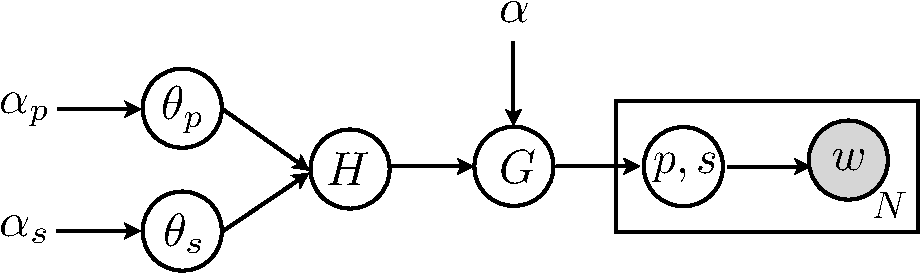
\includegraphics[width=0.6\textwidth]{fig/v2}
\caption{Goldwater model recast as DPMM}
\label{fig:v2}
\end{figure}

\subsection{Parallelizing the DPMM}

While DP mixture models are flexible and allow modelers to sidestep
the issue of model selection, they come at a significant computational
price. The CRP, by itself, requires a full sweep through the full data
for each iteration. Furthermore, in practice, resampling the table
assignment for each data point requires updating several data
structures that keep track of the ``tables'' and ``customers'' of the
restaurant at each state. Depending on the size of the data and how
these data structures are implemented, doing inference in a DP mixture
model can be difficult to scale.

There has been recent interest in the machine learning community in
designing ways to speed up inference in models using the DP. We
briefly review some of the more popular approaches in recent
literature, which have been compiled and described in
\cite{williamson2013}.

Sequential Monte Carlo methods are approximate inference methods that
use swarms of independent, weighted particles to approximate the
posterior distribution of interest, and have been recently applied to
DPs \cite{fearnhead2004, ulker2010, rodriguez2011, ahmed2011}. Since
each particle is independent, such methods are ideal for
parallelization. \cite{williamson2013} note, however, that such
methods can lead to high variance in the approximation, which can be
solved using a resampling step at the cost of introducing dependencies
between particles.

Another method for parallelizing inference in models using the DP is
to use a variational approximation. Since variational approximations
approximate the true posterior with a distribution $q$ that assumes
many simplifying independence assumptions, such approximations can be
easily spread across a cluster and updated in parallel. Such methods
have been explored for both the DP and Hierarchical DP by
\cite{blei2004, kurihara2007, teh2008, wang2011}.

Finally, the MCMC procedures for doing inference in a DP can be
approximated by splitting the computation for sampling table
assignments for each data point across $P$ processors. When sampling a
new assignment for a data point on cluster $P_j$ for $j \in \{1,
\ldots, |P|\}$, we simply consider the assignments of all data points
on processor $P_j$, and use the last known assignment of the data
points on all other processors. Each processor's knowledge of other
assignments is occasionally updated via a global synchronization
step. This approach was explored by \cite{asuncion2008}, but
\cite{williamson2013} note that this method can often be slow to
converge in practice and that it is difficult to know when clusters on
different processors should be split or merged.

The method proposed by \cite{williamson2013} is an improvement over
those presented above in that it builds on a principled extension of
the DP mixture model. At a high level, the mixture model is described
as a finite mixture over several local DPMMs, where each of the random
measures over clusters shares a single Dirichlet process $DP(\alpha,
H)$. This formulation introduces independencies between data points
that are not generated from the same local DPMM, which allows the
seating assignments to be resampled simultaneously in each DPMM. Since
each DPMM can be resampled independently of the others, several CRPs
can be run in parallel across several compute
nodes. \cite{williamson2013} show that this model results in the exact
same marginal distribution over the data $X^n$, and does not depend on
any approximations. The generative story of this model is the
following.

\begin{align*}
  \phi &\sim Dir(\frac{\alpha}{P}, \ldots, \frac{\alpha}{P}) \\
  G_j &\sim DP(\frac{\alpha}{P}, H) \\
  \pi_i \sim \phi,
  \theta_i &\sim G_{\pi_i},
  x_i \sim f(\theta_i)
\end{align*}

where $\phi$ is a categorical distribution over the $P$ processors,
$\alpha$ is the concentration parameter that we would use in the
unparallelized version of the model, $H$ is the base distribution, $j$
ranges over the processor indicators (i.e. $j \in \{1, \ldots, P\}$),
and $i$ ranges over the data indices (i.e. $i \in \{1, \ldots, n\}$).
